\documentclass[a4paper]{article}

\usepackage[english]{babel}
\usepackage[utf8x]{inputenc}
\usepackage{amsmath}
\usepackage{graphicx}
\usepackage{algorithm}
\usepackage{algorithmicx}
\usepackage{algpseudocode}
\usepackage{url}
\renewcommand{\algorithmicforall}{\textbf{for each}}
\let\ForEach\ForAll

\title{ParMA Partition Improvement with Ghosting}

\author{Cameron W. Smith, Gerrett Diamond, Dan Ibanez}

\date{\today}

\begin{document}
\maketitle

\section{Problem Description}

A climate application's pre-processor has a runtime proportional to the number of owned elements plus the number of ghost elements in three ghosting layers; the ghost bridge entity is an edge.  2D meshes of the ocean surface are created using Spherical Centroidal Voronoi Tesselations ~\cite{JuRingler2011,ringler2008}.  The goal is to partition this mesh such that Equation~\ref{eqn:costFn} is minimized while maintaining a low edge cut.  Here the notation $M^d$ is a mesh element and $gM^d$ is a ghost mesh element.
\begin{equation}
\label{eqn:weightVoroni}
w(p_i) = \sum_{M^d \in p_i}w(M^d) + \sum_{gM^d \in p_i}w(gM^d)
\end{equation}
\begin{equation}
\label{eqn:costFn}
I = \frac{max(w(p))}{avg(w(p))}
\end{equation}
Most partitioners cannot account for the ghosted elements as the affect of the ghosts on $w(p_i)$ changes with the partitioning of the owned elements.  

Figure~\ref{fig:ghostEx} depicts an example of three layer ghosting in a simple triangular mesh.

\begin{figure} 
\centering
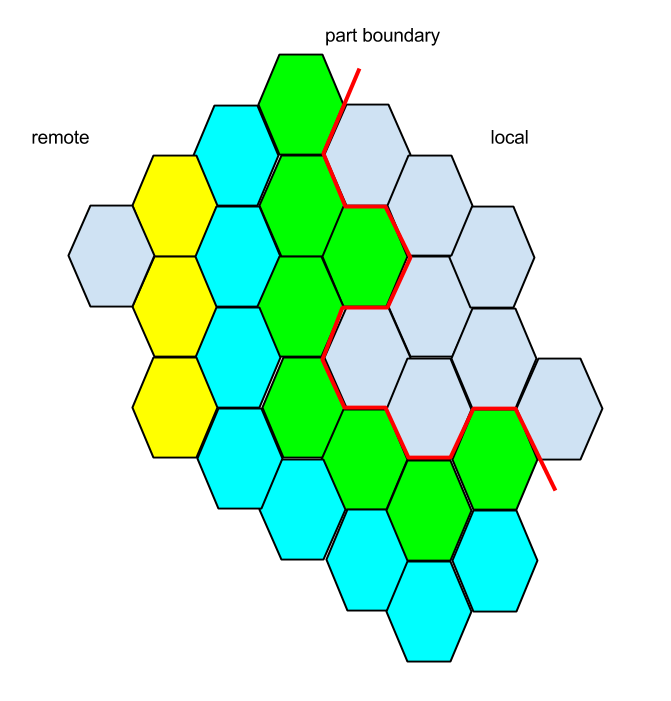
\includegraphics[width=0.4\textwidth]{ghostingExample.png}
\caption{\label{fig:ghostEx} Three layers of elements ghosted from the remote part to the local part.  The first layer is colored green, the second blue, and the third yellow.}
\end{figure}

\section{Approach}

ParMA diffusive partition improvement procedures can account for the ghosted layers using a combination of existing element selection criteria and an extended 'weight' tracking mechanism.  The weight tracking extension relies on the exact knowledge of the change to the ghosted elements as elements on a heavy part are selected for migration to a light part.

ParMA will be ran on the Delaunay triangularization of the Voronoi mesh (Figure~\ref{fig:delaunay}), as depicted in Figures~\ref{fig:NA240}, and will accordingly target vertex balance.  The vertex part assignments, along with identifier information, will be output for partitioning the Voronoi mesh. Vertices in the initial partition are identified by their part number and local vertex number.  Details on the meshes of interest are available online ~\cite{climateMesh}. 

\begin{figure} 
\centering
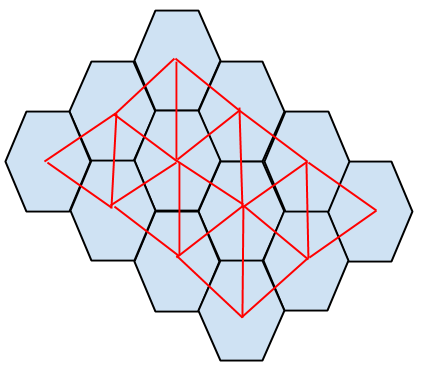
\includegraphics[width=0.4\textwidth]{ghostingOwnershipFig1.png}
\caption{\label{fig:delaunay} A Voronoi diagram and its Delaunay triangularization (in red).}
\end{figure}

\begin{figure}
\centering
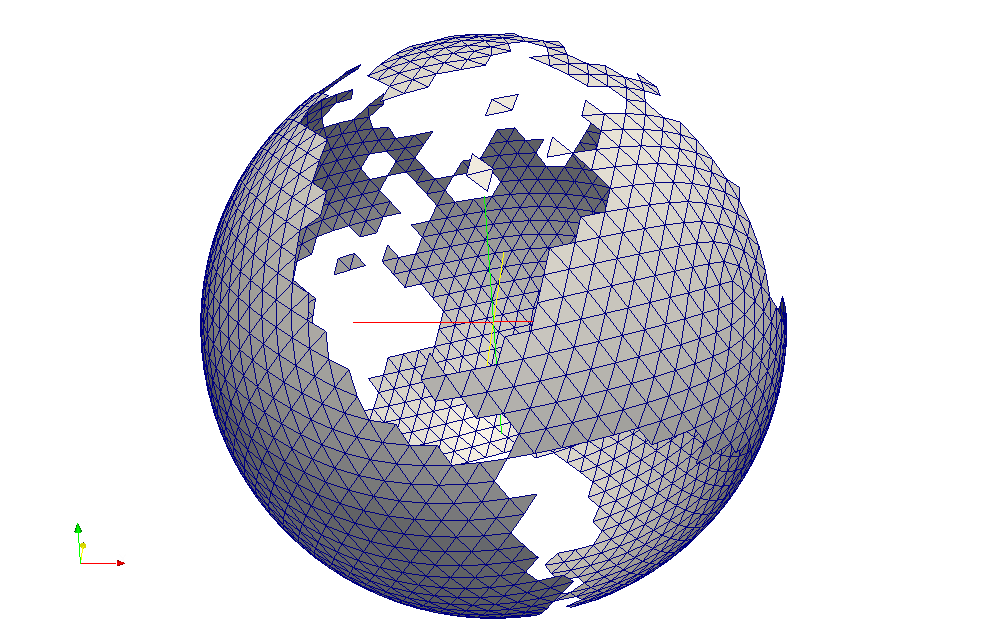
\includegraphics[width=0.75\textwidth]{ocean_QU_240kmNA.png}
\caption{\label{fig:NA240} 240km resolution dual mesh.}
\end{figure}

A Delaunay mesh vertex based partitioning, as depicted in Figure~\ref{fig:ownership2}, is not a valid partition of the Delaunay mesh as each element needs to be assigned to exactly one part.  To obtain unique element assignment an element based partitioning of the Delaunay mesh is performed.  Duplicate Delaunay vertices created on the part boundary as a result of the element partitioning are depicted in Figure~\ref{fig:ownership3} by dotted lines.  These vertex copies in the Voroni mesh this correspond to an element assigned to multiple parts.  Unique part assignment of the Voroni mesh elements is through the ownership associated with the Delaunay mesh vertices.  In Figure~\ref{fig:ownership3} ownership of a mesh vertex is depicted through a colored Voroni element.  Using vertex ownership the weight of each part is defined in Equation~\ref{eqn:weightDelaunay}; the notation $M^0$ is a mesh vertex, $gM^d$ is a ghost mesh vertex, and $\hat{M^0}$ denotes the owned copy of the vertex.
\begin{equation}
\label{eqn:weightDelaunay}
w(p_i) = \sum_{\hat{M^0} \in p_i}w(\hat{M^0}) + \sum_{gM^0 \in p_i}w(gM^0)
\end{equation}

In the Voroni mesh the bridge entity is an edge and three layers of ghosts are needed.  For each shared Voroni mesh edge there is a Delaunay mesh edge connecting Delaunay mesh vertices.  Ghost Delaunay mesh vertices are located using a edge-depth three BFS with root nodes defined as owned Delaunay mesh vertices classified on the partition model boundary.  As with non-ghost Delaunay mesh vertices, each Delaunay mesh ghost vertex corresponds to a Voroni mesh element.  In Figure~\ref{fig:ownership4} the ghost depth is one and green elements are ghosted to the bottom part and yellow elements ghosted to the top part.  The first layer of vertices to be ghosted is formed by (1) the owned vertices classified on the part boundary and (2) vertices edge-adjacent to un-owned vertices classified on the part boundary.

Algorithm~\ref{alg:parma} outlines the top-level procedure for iterative diffusion that seeks to reduce $I$.  While the mesh peak imbalance $I$ is greater than the specified target imbalance a diffusive iteration is executed.  Each iteration first requires finding neighboring parts, computing part weights and exchanging those weights with neighboring parts, finding the elements ghosted on the part boundaries and exchanging the weight of those ghosts with neighboring parts, and lastly computing the amount of weight to migrate to each neighbor.  

Once the Delaunay triangularization is balanced, it is to be converted back into the original format. A single file that lists each vertex's part numbers in the original order must be created. The write function of algorithm~\ref{alg:mpas} describes the steps for creating this file. First each part exchanges vertex info such that each part, $p$, has an equal share of the vertices, $v$, that range from $p*v-p*(v+1)$. Then each part searches for any verticies that were removed during the read operation. Finally, blocks of parts each write to a different file which can then be combined in order to make the final part file.

\begin{figure} 
\centering
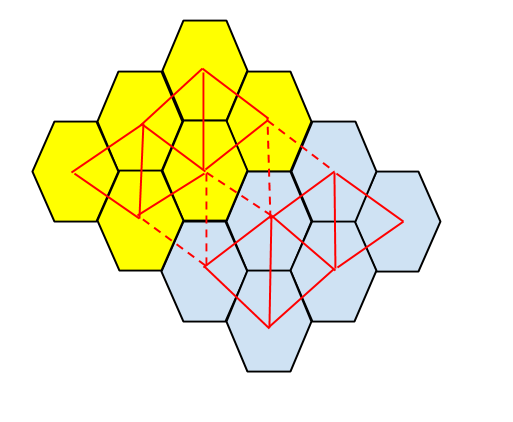
\includegraphics[width=0.4\textwidth]{ghostingOwnershipFig2.png}
\caption{\label{fig:ownership2} A Delaunay mesh vertex based partitioning is not a valid partition of the Delaunay mesh as elements, denoted with dashed edges, span the part boundary.  In the SCOREC unstructured mesh tools an element cannot be divided between multiple parts.}

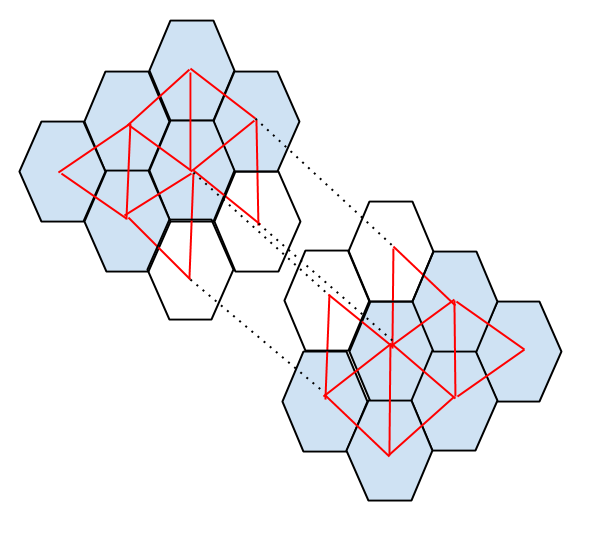
\includegraphics[width=0.4\textwidth]{ghostingOwnershipFig3.png}
\caption{\label{fig:ownership3} An element based partitioning of the Delaunay mesh with duplicate Delaunay vertices on the part boundary.  Owned Delaunay mesh vertices are marked with colored Voroni elements.}

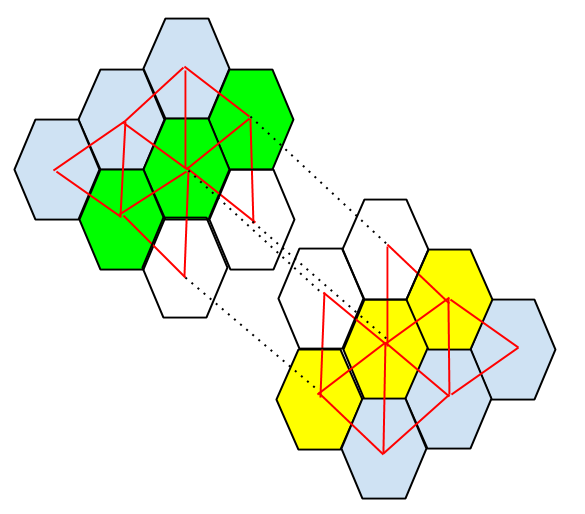
\includegraphics[width=0.4\textwidth]{ghostingOwnershipFig4.png}
\caption{\label{fig:ownership4} One layer edge-based ghosting of a Delaunay mesh element partition.  Green elements are ghosted to the bottom part and yellow elements ghosted to the top part.}
\end{figure}

\begin{algorithm}
\caption{ParMA Ghosting improvement}
\label{alg:parma}
\begin{algorithmic}[1]
\Require {mesh $M$ of dimension $d$, bridge ent dim $bDim$, num ghost layers $layers$}
\Procedure{parma}{$M$, $bDim$, $layers$}
  \While {$imbalance > tolerance$}
    \State $nbors \leftarrow findNeighbors()$
    \State //part weight only includes owned vertices
    \State $weight \leftarrow exchangeWeights(nbors)$
    \State //part weight only includes owned vertices
    \State $ghost \leftarrow exchangeGhostWeights(nbors)$
    \State $tgts \leftarrow computeTargets(weight, ghost)$
    \State $diffuse(tgts)$
  \EndWhile
\EndProcedure

\Procedure{diffuse(targets)}{}
  \State $plan \leftarrow \emptyset$
  \ForEach {$vtx \in boundaryVertices$}
    \State $neighbor \leftarrow getNeighbor(elm)$
    \If { $tgts.has(neighbor)$ AND $plan(neighbor) < tgts(neighbor)$}
      \If {meets selection criteria}
        \State $plan.add(elm)$
      \EndIf 
    \EndIf
  \EndFor
  \State $migrate(plan)$
\EndProcedure
\end{algorithmic}
\end{algorithm}

\begin{algorithm}
\caption{MPAS I/O}
\label{alg:mpas}
\begin{algorithmic}[1]
%\Require {mesh $M$ of dimension $d$, bridge ent dim $bDim$, num ghost layers $layers$}
\Procedure{read}{}
  
\EndProcedure

\Procedure{write}{}
  \State $vtxs \leftarrow \emptyset$
  \ForEach {$owned vtx$}
    \State send vtx number and part number to target
  \EndFor
  \ForEach {$recieved vtx$}
    \State $vtxs[vtx number] \leftarrow $
  \EndFor
  \ForEach {$vtx number$}
    \If {vtxs[vtx number] is empty}
      \State $vtxs[vtx number] \leftarrow random part number$
    \EndIf
  \EndFor
  \State Open file 
  \ForEach {$v \in vtxs$}
    \State $file \leftarrow part number$
  \EndFor
\EndProcedure
\end{algorithmic}
\end{algorithm}

\begin{figure} 
\centering
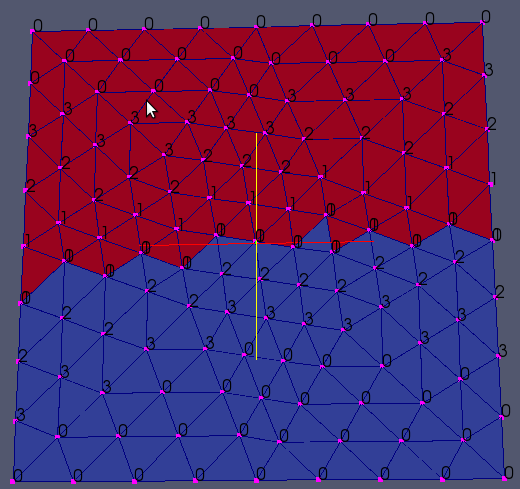
\includegraphics[width=0.8\textwidth]{plateghosts.png}
\caption{\label{fig:ownership4} Three layers of ghosting between two parts of a test mesh.  The boundary is only ghosted from the part that owns the vertices to the not owned part.}
\end{figure}

\section{Results}

The 500K element North America graded 15km to 75km, and the 3.6M element 15km uniform meshes are partitioned with Zoltan local and global ParMETIS, and ParMA RIB to a 5\% peak element imbalance and then ParMA ghost balancing is applied. 
Tests were ran on RPI's AMOS and ALCF's Cetus, and Mira IBM BlueGene/Q systems.  
Tables ~\ref{tab:nalg}, \ref{tab:nagg} and \ref{tab:naplrib} list the timings to compute the partition, migrate the elements, the resulting initial ghost imbalance, $I_0$, the final ghost imbalance, $I_N$, the number of ghost balancing iterations, $N$, and the total ghost balancing time for the North America graded mesh.
Likewise, results for the 15km uniform mesh are listed in Tables ~\ref{tab:15kmlg}, \ref{tab:15kmgg} and \ref{tab:15kmplrib}.  
Note, the 15km 6144 partition was ran using a combination of threads and MPI processes (COMING SOON) to accommodate the BlueGene/Q's power of two process per node requirement; all other ghost balancing tests were ran without threads.

Figure~\ref{fig:60km0_255} and \ref{fig:60km384_404} respectively depict the initial ParMA RIB partition and the resulting ghost balanced partition.  
The ghost balanced partition maintains the original partitions low degree while smoothing out the part boundaries via a high surface area vertex selection mechanism discussed in ~\cite{ParMA-2014}.

\begin{figure} 
\centering

\includegraphics[width=0.45\textwidth]{60km/init/0_255.png}

\includegraphics[width=0.5\textwidth]{60km/final/0_255.png}
\caption{\label{fig:60km0_255} RIB initial partition (left) and the ParMA ghost balanced partition (right).}

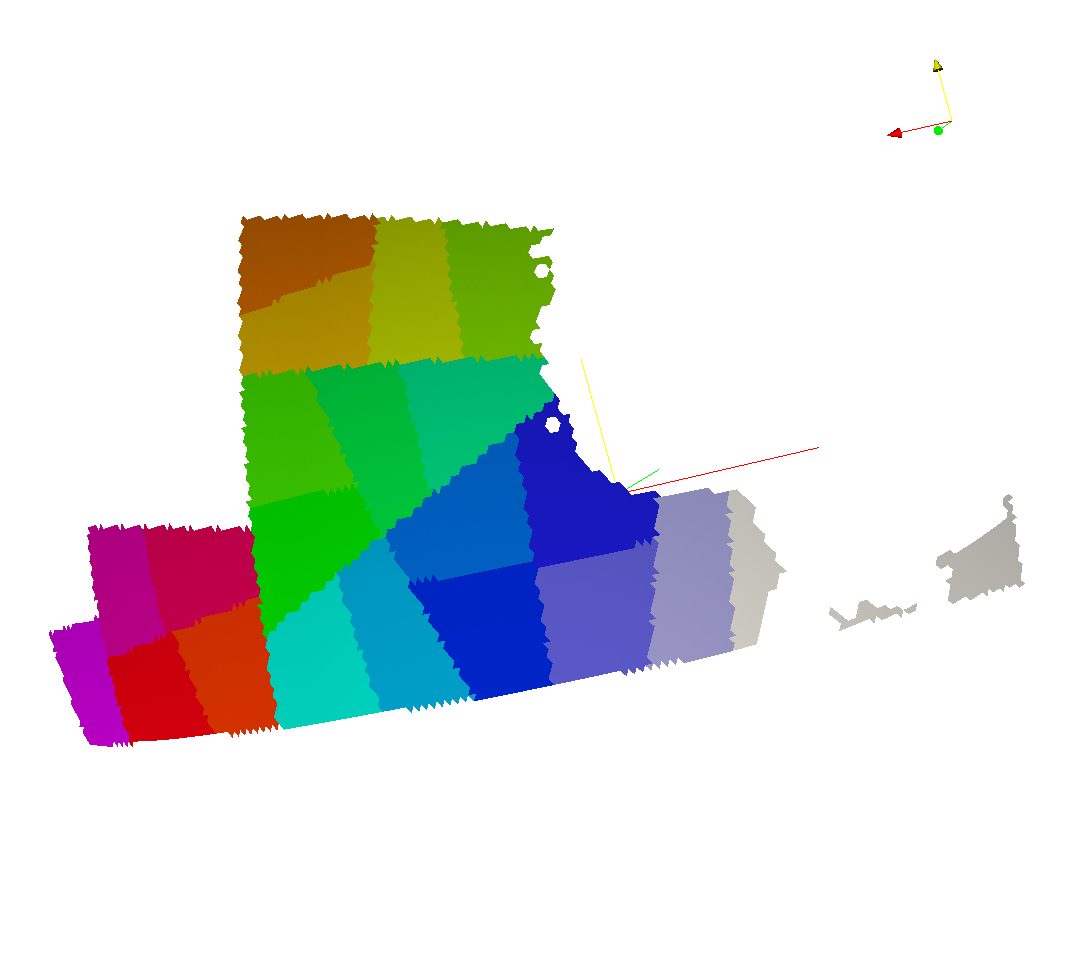
\includegraphics[width=0.6\textwidth]{60km/init/384_404.png}
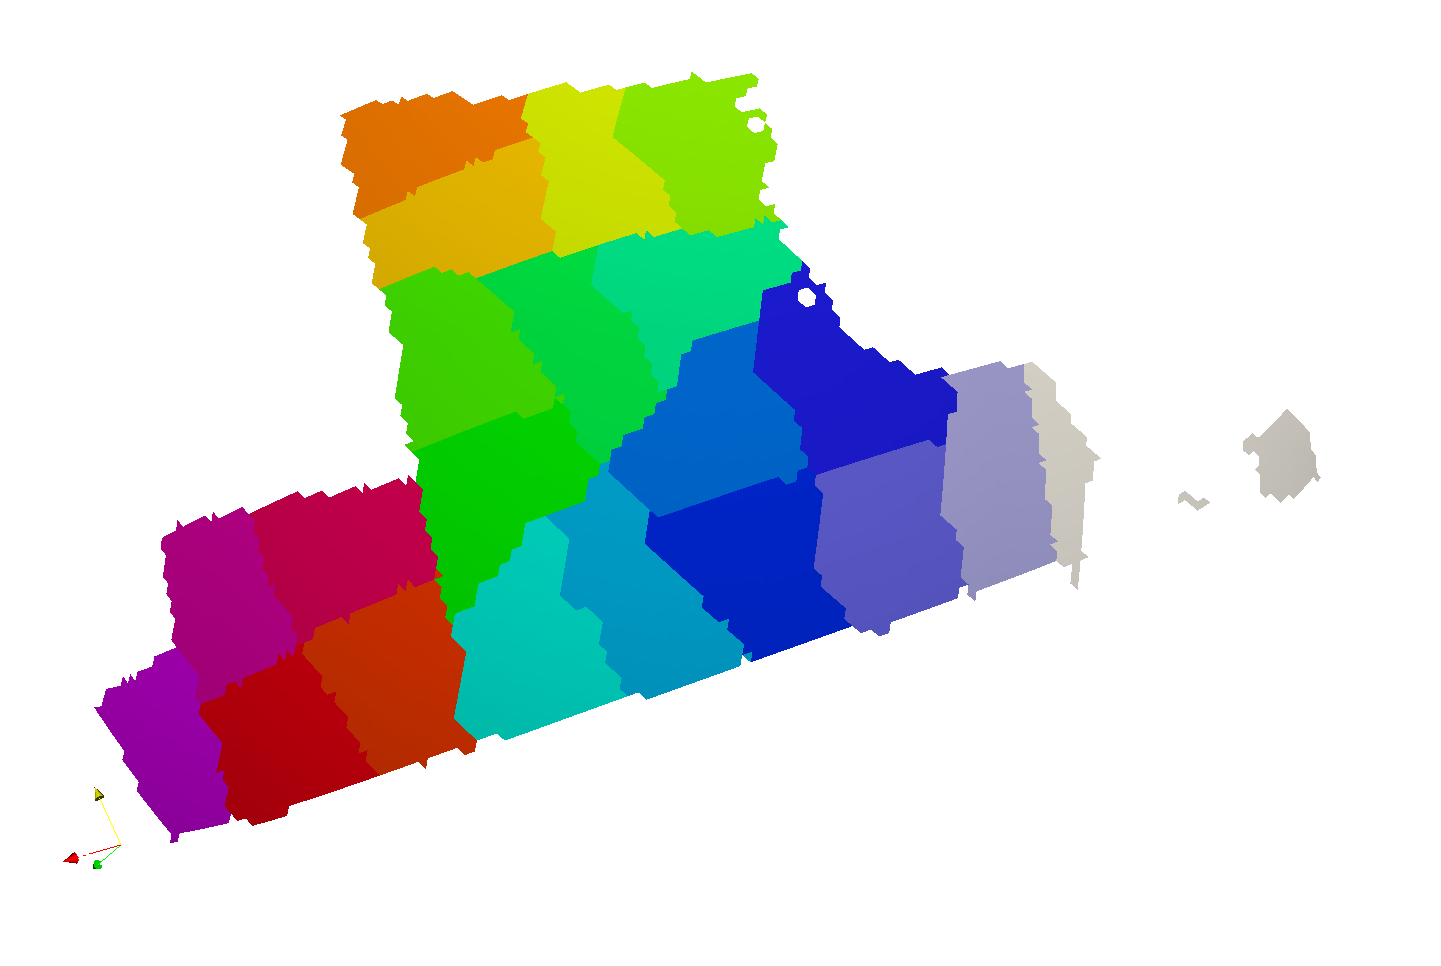
\includegraphics[width=0.6\textwidth]{60km/final/384_404.png}
\caption{\label{fig:60km384_404} RIB initial partition (top) and the ParMA ghost balanced partition (bottom).}
\end{figure}

\begin{table}
\centering
\caption{\label{tab:nalg}North America Graded: Zoltan Local ParMETIS followed by ghost balancing.}
\begin{tabular}{  l | l | l | l | l | l | l | l | l | l | l }
    \hline
    nodes & parts & tgt parts & factor & plan (s) & migrate (s) & total (s) & $I_0$ & $I_N$ & N & time (s) \\ \hline
    32 & 1 & 32 & 32 & 31.73 & 92.35 & 124.07 & 1.048 & 1.048 & 0 & 0.10 \\ 
    32 & 32 & 512 & 16 & 1.01 & 2.38 & 3.39 & 1.218 & 1.05 & 29 & 0.98 \\ 
    32 & 32 & 1024 & 32 & 1.10 & 3.24 & 4.34 & 1.236 & 1.046 & 32 & 1.07 \\ 
    32 & 32 & 2048 & 64 & 1.26 & 4.63 & 5.90 & 1.276 & 1.05 & 112 & 4.95 \\ 
\end{tabular}

\caption{\label{tab:nagg}North America Graded: Zoltan Global ParMETIS followed by ghost balancing.}
\begin{tabular}{  l | l | l | l | l | l | l | l | l | l | l }
    \hline
    nodes & parts & tgt parts & factor & plan (s) & migrate (s) & total (s) & $I_0$ & $I_N$ & N & time (s) \\ \hline
    32 & 1 & 32 & 32 & 31.73 & 92.35 & 124.07 & 1.048 & 1.048 & 0 & 0.10 \\ 
    32 & 32 & 512 & 16 & 1.97 & 2.38 & 4.34 & 1.179 & 1.049 & 31 & 1.05 \\ 
    32 & 32 & 1024 & 32 & 2.86 & 3.07 & 5.93 & 1.204 & 1.05 & 28 & 0.93 \\ 
    32 & 32 & 2048 & 64 & 4.65 & 5.19 & 9.84 & 1.281 & 1.046 & 92 & 4.14 \\ 
\end{tabular}

\caption{\label{tab:naplrib}North America Graded: ParMA local RIB followed by ghost balancing.}
\begin{tabular}{  l | l | l | l | l | l | l | l | l | l | l }
    \hline
    nodes & parts & tgt parts & factor & plan (s) & migrate (s) & total (s) & $I_0$ & $I_N$ & N & time (s) \\ \hline
    32 & 1 & 32 & 32 & 11.27 & 90.34 & 101.61 & 1.079 & 1.048 & 6 & 0.98 \\ 
    32 & 32 & 512 & 16 & 0.25 & 2.32 & 2.56 & 1.27 & 1.05 & 15 & 0.50 \\ 
    32 & 32 & 1024 & 32 & 0.29 & 3.21 & 3.49 & 1.443 & 1.045 & 25 & 0.81 \\ 
    32 & 32 & 2048 & 64 & 0.33 & 4.68 & 5.01 & 1.394 & 1.046 & 38 & 1.62 \\ 
\end{tabular}

\caption{\label{tab:15kmlg}15km Uniform: Zoltan local ParMETIS followed by ghost balancing.}
\begin{tabular}{  l | l | l | l | l | l | l | l | l | l | l }
    \hline
    nodes & parts & tgt parts & factor & plan (s) & migrate (s) & total (s) & $I_0$ & $I_N$ & N & time (s) \\ \hline
    1 & 1 & 8 & 8 & 26.04 & 195.83 & 221.87 & 1.008 & 1.008 & 0 & 1.78 \\ 
    8 & 8 & 64 & 8 & 27.80 & 57.08 & 84.88 & 1.019 & 1.019 & 0 & 0.31 \\ 
    8 & 64 & 512 & 8 & 3.52 & 15.26 & 18.78 & 1.073 & 1.048 & 6 & 0.55 \\ 
    128 & 512 & 1024 & 2 & 0.43 & 0.76 & 1.20 & 1.116 & 1.048 & 11 & 0.70 \\ 
    128 & 512 & 2048 & 4 & 0.44 & 0.90 & 1.34 & 1.17 & 1.049 & 14 & 0.78 \\ 
    128 & 512 & 4096 & 8 & 0.46 & 1.01 & 1.47 & 1.207 & 1.05 & 21 & 0.96 \\ 
    128 & 512 & 6144 & 12 & 0.48 & 1.08 & 1.55 &  &  &  &  \\ 
\end{tabular}

\caption{\label{tab:15kmgg}15km Uniform: Zoltan global ParMETIS followed by ghost balancing.}
\begin{tabular}{  l | l | l | l | l | l | l | l | l | l | l }
    \hline
    nodes & parts & tgt parts & factor & plan (s) & migrate (s) & total (s) & $I_0$ & $I_N$ & N & time (s) \\ \hline
      1 & 1 & 8 & 8 & 26.04 & 195.83 & 221.87 & 1.008 & 1.008 & 0 & 1.78 \\ 
      8 & 8 & 64 & 8 & 32.40 & 62.70 & 95.09 & 1.052 & 1.048 & 2 & 0.78 \\ 
      8 & 64 & 512 & 8 & 4.74 & 8.88 & 13.62 & 1.126 & 1.049 & 14 & 1.26 \\ 
      128 & 512 & 1024 & 2 & 1.13 & 1.44 & 2.56 & 1.131 & 1.05 & 23 & 1.46 \\ 
      128 & 512 & 2048 & 4 & 1.42 & 1.34 & 2.76 & 1.152 & 1.048 & 16 & 0.88 \\ 
      128 & 512 & 4096 & 8 & 2.07 & 1.21 & 3.27 & 1.202 & 1.049 & 23 & 1.04 \\ 
      128 & 512 & 6144 & 12 & 2.63 & 1.19 & 3.82 &  &  &  & \  \\ 
\end{tabular}

\caption{\label{tab:15kmplrib}15km Uniform: ParMA local RIB followed by ghost balancing.}
\begin{tabular}{  l | l | l | l | l | l | l | l | l | l | l }
    \hline
    nodes & parts & tgt parts & factor & plan (s) & migrate (s) & total (s) & $I_0$ & $I_N$ & N & time (s) \\ \hline
      1 & 1 & 8 & 8 & 34.24 & 126.62 & 160.85 & 1.007 & 1.007 & 0 & 1.83 \\ 
      8 & 8 & 64 & 8 & 7.01 & 51.85 & 58.86 & 1.054 & 1.047 & 3 & 1.17 \\ 
      8 & 64 & 512 & 8 & 0.80 & 6.88 & 7.67 & 1.127 & 1.047 & 13 & 1.19 \\ 
      128 & 512 & 1024 & 2 & 0.05 & 0.71 & 0.76 & 1.182 & 1.049 & 17 & 1.11 \\ 
      128 & 512 & 2048 & 4 & 0.07 & 0.88 & 0.95 & 1.212 & 1.049 & 24 & 1.30 \\ 
      128 & 512 & 4096 & 8 & 0.09 & 0.96 & 1.05 & 1.267 & 1.046 & 33 & 1.38 \\ 
\end{tabular}
\end{table}

\section{Code}

The source can be downloaded from the following github repo \\
https://github.com/SCOREC/core

The code in parma/diffMC/src/parma\_ghost.cc implements the partitioning procedures and test/ghost.cc provides a test driver.  The test driver can be built with the command `make ghost'.  In the plate/2 directory of the test meshes SVN repo http://redmine.scorec.rpi.edu/svn/meshes is a two part 2D mesh for testing.  This mesh is classified on the plate/plate.dmg model.  Run the driver with the command `mpirun -np PROCS ./ghost MODEL MESH'.

The code in mpas/apfMPAS.cc implements NetCDF to SCOREC and SCOREC to NetCDF protocols and test drivers are in test/mpas\_read.cc and test/mpas\_write.cc. These test drivers can be built using 'make mpas\_read' and 'make mpas\_write' respectively. First run mpas\_read with './mpas\_read NetCDF OUT\_MESH OUT\_MODEL'. After reading the NetCDF file the SCOREC mesh must be split to desired part count using the split program, built with 'make split' and ran with './split MODEL MESH SPLIT\_MESH FACTOR'. To write graph.info.part.\# files for the newly balanced mesh run 'mpirun -np PROCS ./mpas\_write MODEL MESH NetCDF'.

\newpage
\bibliographystyle{plain}
\bibliography{references.bib}


\end{document}


